%!TEX root=../book.tex

\chapter{One-Way ANOVA}

\section{Overview of One-Way ANOVAs}

To understand ANOVAs, let's think back once more to \textit{t}-tests. There, we're looking to determine whether there is a difference between the means of two samples of data. But that if we want to look at more than two groups? 

Well, using what we've learned up to now, we're stuck: there's nothing more we can do. But of course that's not \textit{really} the case, is it? Otherwise we wouldn't be writing this chapter!

The idea with a one-way ANOVA is that we have a variable of interest, but three or more levels of our grouping variable. For instance, we might be looking at student test scores as a function of classroom type: regular, honors, AP (advanced placement), or IB (international baccalaureate). That's way beyond the scope of any \textit{t}-test that we've come across. Thankfully, though, the ANOVA is happy to step in to fill the gap.

Before we can actually run the test, however, there is some background information that we need to understand first.

\subsection{Fixed and Random Effects}

For starters, we should be familiar with fixed, random, and mixed effects models. Broadly speaking, these refer to how the treatment factors are defined within the context of the experiment.

One caveat before we get started, though: there is no single agreed-upon definition for fixed and random effects. Rather, the precise definition is going to depend on the exact context of your experiment and your program of research. For a quick overview of these different definitions (or at least a spattering of them), check out \href{http://andrewgelman.com/2005/01/25/why_i_dont_use/}{Andrew Gelman's write-up, linked here}.

\subsubsection{Fixed Effects}

In a fixed-effects model, there is a basic assumption that the individual-specific effect is correlated with the independent variable(s). The idea here is that person-to-person, there is little variance beyond that caused by the treatment effect.

\subsubsection{Random Effects}

Random effects models assume that there is some inherent amount of individual variance not accounted for by the treatment. So if we were talking about a regression equation with a random intercept $a_i$ and fixed slope $b$, each individual would have his or hew own regression line, parallel to every other individual but with a differing intercept (cf. Figure \ref{fig:anova01}).

\begin{figure}[h]
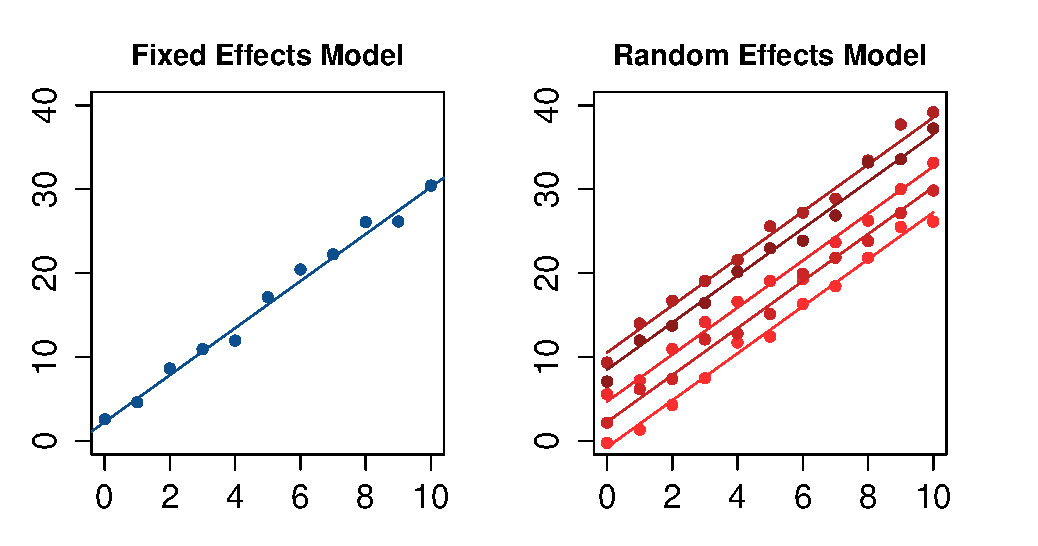
\includegraphics[width=35pc]{anova01}
\caption{A regression equation assuming fixed-effects factors for all individuals (left) and a random-effects intercept for 5 individuals (right).}
\label{fig:anova01}
\end{figure}

\subsection{Sum of Squares}

Residual, treatment, and total sums of squares are discussed more fully in our chapter on simple linear regression.

\subsection{The F-Test}

\subsection{Recommended Legwork}

\subsubsection{Power Analyses}

\subsubsection{Effect Size}

\subsection{Follow-Up Analyses}

\subsubsection{Post-Hoc Tests}

\subsubsection{Planned Comparisons and Linear Contrasts}

\section{Cautions and Considerations}

\subsection{Assumptions}

\subsection{Robustness of the Test}

\section{Implementation in R}

\subsection{aov() vs. lme() vs. lmer()}

\section{Case Study: [STUDY]}

\section{Exercises}

\section{Additional Resources}

